%Group Report Information: Did it work properly? What kind of tests did you run to test your prototype? Could you provide some data that shows the performance of the prototype (speed, success rate, etc.)?
\section{Results/Analysis}
The first time after having assembled all the different parts and placed it on a whiteboard we started testing, moving both motors around 100 steps. This was a success and the line seemed to be straight. We later found out that the line was only straight because we had placed the pen in the middle of the two motors (equal line length). If the line lengths were not equal, hence the pen not being exactly in the middle, the drawn line would have an angle towards the middle. This meant that there was an issue in our understanding of the math. In particular we would trouble drawing anything accurately relatively. We needed to know all sides of the triangle to then use an absolute positioning. We also believed that we could somehow calculate the length between {\it MR} and {\it ML}. This mistake only came up when we began to program the software part after having produced much of the prototype. The solution was to assume a fixed length between {\it MR} and {\it ML}. The results are also skewed as a result of the magnets for homing (endstop) not being close enough to the end of the line. After adding homing and not being accurate on the numbers needed for absolute positioning, we observe the consequence quite noticeable on figure \ref{SkewedDrawing} where the supposed circle becomes an oval. This is a problem with accuracy as the machine keeps hitting the same place when it wants to reach a coordinate, but it is not always the correct coordinate. Therefore, our drawing machine has reached a medium accuracy and a higher precision (medium because it is clearly still high enough that one can make out what it is drawing in most cases, exceptions being that circles becomes ovals etc.).
\\\\
This is what lead to us using a fixed length between the motors and also enforce homing. \\ %kan du beskrive det bedre måske?
We moved on to adding sensors and the homing software to better define the canvas. This made it possible to control the tests as we would have the same canvas each time. We then started testing diagonal lines with success and moved on to draw a circle. See a video of the first circle drawn: \url{https://youtu.be/KyW-_ZQY8U0}.\\
The video shows how the drawing head first {\it home}, then finds the center of the canvas and draws a circle. The result was a circle though closer to egg shaped. \\
We went on to challenge the Drawing Machine further with our third goal, being uploading an image. We found a picture of a skull in a circle with the text "Please Don't Touch". The process of drawing the skull image can be seen in the appendix \cref{fig:Images/Jacobselskovsbilleder/IMG 2035.jpg,fig:Images/Jacobselskovsbilleder/IMG 2036.jpg,fig:Images/Jacobselskovsbilleder/IMG 2038.jpg,fig:Images/DrawingMachine/SkewedDrawing.jpg} the picture was rotated and flipped. Testing with a diagonal line from corner to corner, we could see that origo, $(0,\ 0)$, was in the top left hand corner, which is the same used by {\it PIL}, therefore, the mismatch likely happens in the segmentation code that we wrote. However, instead of trying to debug we simply applying the inverted functions to the input image before creating the list of coordinates to draw in the segmentation algorithm, the result. This had the small implication that transport lines now went from top to bottom instead of left to right, an example of drawing with vertical transport lines is especially seen in the text in \cref{fig:ost}.

\begin{figure}[H]
    \caption{Configuring bridging between drawing machine and logic}
    \begin{subfigure}[t]{.24\textwidth}
        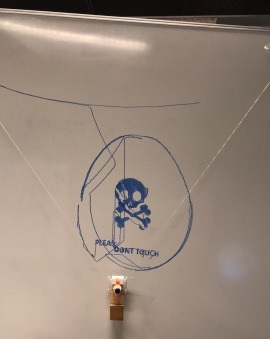
\includegraphics[width=\textwidth]{Images/DrawingMachine/SkewedDrawing.jpg}
        \caption{Drawing machine skewed drawing.}
        \label{SkewedDrawing}
        \centering
    \end{subfigure}
    \begin{subfigure}[t]{.24\textwidth}
        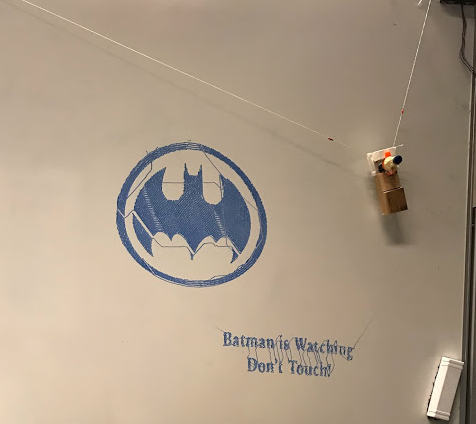
\includegraphics[width=\textwidth]{Images/Jacobselskovsbilleder/Batman.PNG}
        \caption{Drawing batman logo and text, after inverted operations to input image to counter rotation and flipping}
        \label{fig:ost}
        \centering
    \end{subfigure}
\end{figure}

In the end we tried taking a photo in the way that is seen in \cref{subfig:original}, thus trying to achieve our initial goal of being able to draw from photos. Using OpenCV\cite{itseez2015opencv}, we applied edge detection before feeding the image to our segmentation algorithm, the input image is seen in \cref{fig:test_drawing}. We tried two partially completed experiments of two different neighborhoods. However, in the end both seemed to overdo in terms of transport lines which would blur the actual drawing, see \cref{fig:attempted_drawing}. The reason for the many similar transport lines is reminiscent of how the top right hand corner of \cref{subfig:original} is drawn where there is a grid in the ceiling. In all simulations \crefrange{subfig:3x3}{subfig:100x100}, the grid turns out as one big blob, since the many actual lines were too close to not cross over with transport lines.

\begin{figure}[H]
    \caption{Testing drawing of photographs}
    \begin{subfigure}[t]{.24\textwidth}
    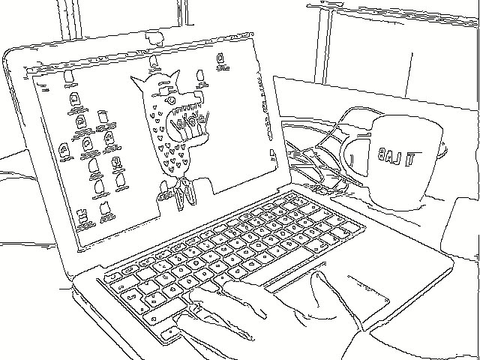
\includegraphics[width=\textwidth]{Images/test_drawing.png}
    \caption{Input image to draw, after applying edge detection}
    \label{fig:test_drawing}
    \end{subfigure}
    \begin{subfigure}[t]{.24\textwidth}
    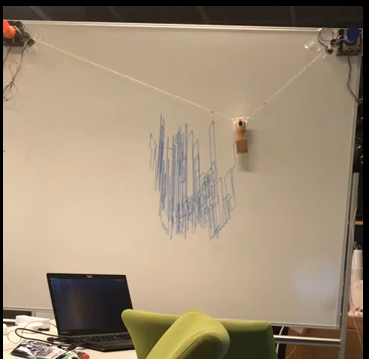
\includegraphics[width=\textwidth]{Images/DrawingMachine/DrawingComputer}
    \caption{The resulting drawing, before terminating the experiment}
    \label{fig:attempted_drawing}
    \end{subfigure}
\end{figure}